\documentclass{article} % For LaTeX2e
\usepackage{nips15submit_e,times}
\usepackage{hyperref}
\usepackage{url}
\usepackage{graphicx}
\usepackage{float}
\usepackage{mathtools}
\usepackage{listings}
\usepackage{bm}
\usepackage{amsmath}
\graphicspath{ {figures/} }
\DeclareMathOperator*{\argmin}{\arg\!\min}
\DeclareMathOperator*{\argmax}{\arg\!\max}
\DeclareMathOperator*{\sigmoid}{sigmoid}
\DeclarePairedDelimiterX{\norm}[1]{\lVert}{\rVert}{#1}

\renewcommand{\lstlistingname}{Listing}

\lstset{
   breaklines=true,
   basicstyle=\ttfamily}

%\documentstyle[nips14submit_09,times,art10]{article} % For LaTeX 2.09


\title{COMPGI15: Information Retrieval \& Data Mining \\
Time Series Forecasting Group Project}


\author{
Rupert Chaplin\\
\texttt{rupert.chaplin.15@ucl.ac.uk} \\
\And
Artemis Dampa\\
\texttt{artemis.dampa.15@ucl.ac.uk} \\
\And
Megane Martinez\\
\texttt{megane.martinez.15@ucl.ac.uk} \\
}


\newcommand{\fix}{\marginpar{FIX}}
\newcommand{\new}{\marginpar{NEW}}

\nipsfinalcopy % Uncomment for camera-ready version

\begin{document}


\maketitle

% No abstract needed
\begin{abstract}
placeholder for abstract
\end{abstract}

\section*{Introduction}
A time series can be defined as a set of observations measured successively over a continuous time interval. Every measurement is taken at a specific time which is equally distant to its subsequent. The analysis of time series takes into consideration the ordering of the data points and constitutes a useful tool in order to extract information such as the causal effect of time change on the variable which is examined. After describing and analysing the time series one can gain an understanding of the data and thus, define a model with the best possible fit at the data based on the past values of the examined variable and/or the past and present observations of other variables which might influence the former. Using the created model one can, finally, make predictions and forecast the future values of the examined variable or even use models to backcast and possibly fill in missing values. The ultimate goal of time series analysis is to control and manage the process involved in the time series.

Load forecasting and especially, short term load forecasting which can predict energy load values ranging from one day to one fortnight at hourly or sub hourly intervals, has always been of great importance for managing power systems. It is used in economic generation scheduling, fuel scheduling, unit commitment and system security, as well as in transmission and distribution operations. There are several machine learning methods which can be applied in order to achieve short term load forecasting, such as ARIMA, Multiple linear regression, Gradient boosting and Neural networks.

The dataset used in order to implement the time series techniques for forecasting (and backcasting) is provided by the Load Forecasting track of Global Energy Forecasting Competition 2012. The aim of the competition was to collect different approaches for energy forecasting in order to “overcome forecasting challenges in the smart grid world”. More specifically, the load forecasting track was addressing a hierarchical load forecasting problem. The goal was to use forecasting (and backcasting) in order to predict hourly loads (in kW) for a US utility with 20 zones.



\section*{Data availability}
In developing this work, we embraced the same constraints on data use imposed upon the original Kaggle challenge - confining ourselves to use of the originally provided datasets, which are:
\begin{itemize}
\item Time series for the electricity load in 20 zones, at hourly intervals between 1 January 2004 and 30 June 2008.
\item Time series of temperature readings at 11 stations, at hourly intervals over the same time period (locations not provided)
\item Dates of US holidays falling during the period
\end{itemize}
The task is to generate estimates of electricity load in each zone, and for the region as a whole, for eight hold out weeks within the period.  Additionally, forecasts are required for the week 1 July 2008 to 7 July 2008, for which no temperature readings are available.

\section*{Temperatures forecasting}
In this project, most of the implemented models, use the values provided in the temperature dataset as features for predicting energy loads values. However, the last week of temperature values is missing (2008-07-01 to 2008-07-01). Therefore, predicting the values for this week was a critical challenge for the results would impact the quality of the results provided by the implemented models.
Teams that took part in the Kaggle competition usually, used naive techniques for forecasting temperature values such as taking the average of the previous values. In this project, it was decided to use ARIMA modelling to forecast the missing temperatures. This approach represents an improvement from what has been done in the Kaggle competition and was one of the challenges to overcome.

\section*{Consideration of feature selection}
Before determining the features of the model and after performing data cleansing and editing, it is essential to create and examine the time plot of the data. The time plot can show the behavior of the data and reveal important features such as seasonal variation and trend which is defined as “an increasing normal number assigned to each observation in chronological order”.

In our case the time plot showed various fluctuations with an annual seasonality which led us to develop a set that combines several features; trend, hour with 24 levels (representing the hours of a day), weekday with seven levels (representing the days of a week), month with 12 levels (representing the months of a year), temperature of the current hour, temperature of the current hour and cubic temperature of the current hour. In addition to those main features, interaction between them was taken into account forming several cross effects; weekday$\times$hour, temperature$\times$month, temperature$^2$$\times$month, temperature$^3$$\times$month, temperature$\times$hour, temperature$^2$$\times$hour and temperature$^3$$\times$hour. After measuring the feature importance, we plotted the results as shown in Figure \ref{fig:var_imp}.
\begin{figure}
  \centering
    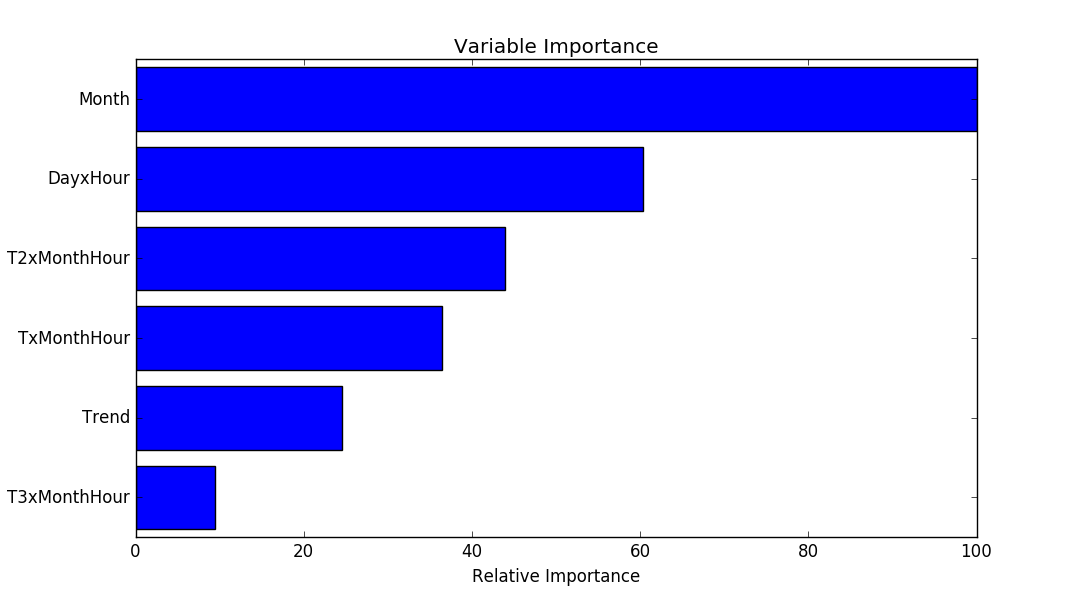
\includegraphics[width=0.80\textwidth]{variable_importance}
  \caption{Shows the feature importance measurements over the features}
  \label{fig:var_imp}
\end{figure}

\section*{Evaluation Methods}
To compare the predictive power of our models, we have adopted the same evaluation method adopted by the original Kaggle competition.  This allows us to objectively compare predictions from the different approaches we consider, and also compare out results to those achieved by those participating in the original competition.

This approach is a Weighted Root Mean Square Error, with a weighting of 1 for each zonal prediction within the period covered by training data, and a weighting of 8 for predictions within the forecast period.  Weightings of 20 and 160 are applied for each prediction of total regional load.

Root Mean Square Error is a common evaluation method for regression problems - it is a measure of average absolute distance between predicted and actual results.  It has the advantage of being expressed in the same units as that of the data we are trying to predict.  Unlike some other approaches, it is indifferent to whether overall discrepancy is due to large discrepancies on a small number of distant outliers, or due to smaller errors affecting a large number of datapoints.

The addition of weighting for this problem means that succesful models will be those which are 

Monitoring the evaluation metric also allows us to monitor models for `overfitting'.  Overfitting occurs when a model becomes tuned to the specific characteristics of a training data set, and does not generalise well to unseen test data. Overfitting would be signalled if the error measure is higher for a test dataset than it is for training data.

\section*{Modelling Approaches}

\subsection*{ARIMA for load forecasting}

\subsection*{ARIMA for temperature forecasting}

\subsection*{Multiple Linear Regression}

\subsection*{Gradient Boosting}
Gradient Boosting is an ensemble learning method which builds additive regression models in a forward stage-wise manner. In each stage it fits a parameterised base learner to the gradient of the loss function which decreases in regard to the model values of every training sample. Gradient boosting can handle and process various data types and many different features. The factor of randomisation of gradient boosting also improves its accuracy and execution speed. Moreover, through its robust loss functions it can eliminate noise by removing outliers and thus, prevent the training model from overfitting to the data samples.

In our approach, a set of features was introduced to the gradient boosting regression model in order to best fit the data. The features are composed by the month (1-12), weekday (1-7), hour (1-24), summer (true-false), trend, holiday falling and the temperature measurements of each of the 11 temperature stations. After training the model the root mean squared error of the testing was generated and was approximately equal to 76676 whilst its weighted root mean squared error was approximately equivalent to 112081. Finally, the error of the training set and test set was computed at each iteration and can be summarised in Figure \ref{fig:deviance}, whilst the importance of all features was measured and can be observed in Figure \ref{fig:boost_imp}.
\begin{figure}
  \centering
    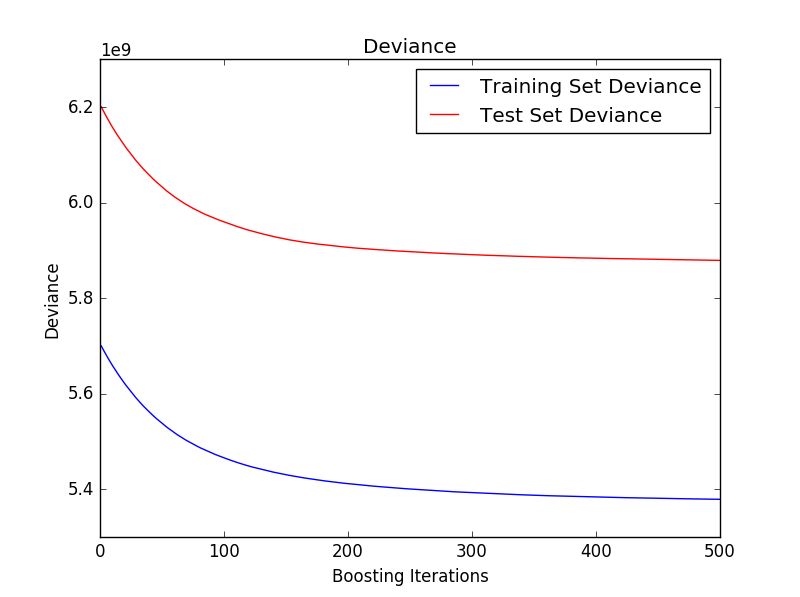
\includegraphics[width=0.80\textwidth]{deviance}
  \caption{Shows the deviance of the training and test set in gradient boosting}
  \label{fig:deviance}
\end{figure}
\begin{figure}
  \centering
    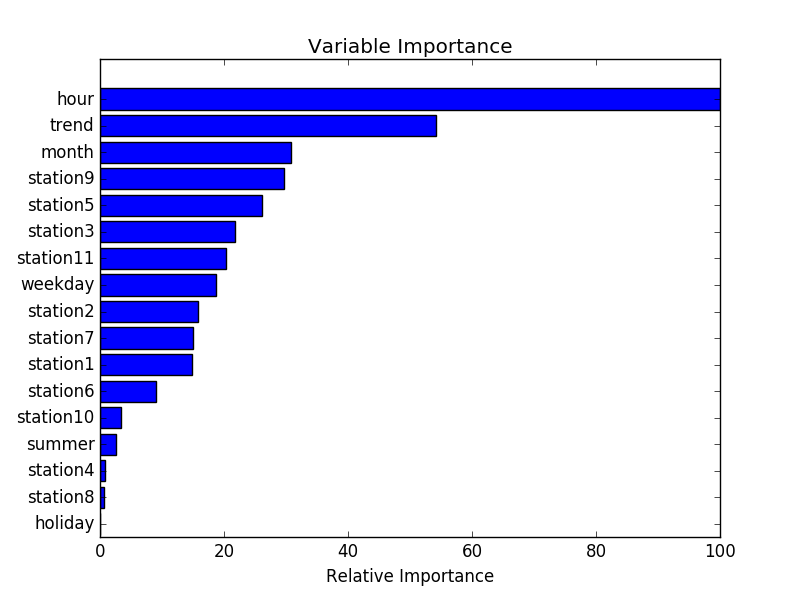
\includegraphics[width=0.80\textwidth]{boost_imp}
  \caption{Shows the feature importance measurements over the features in gradient boosting}
  \label{fig:boost_imp}
\end{figure}


\subsection*{Neural Networks}

\section*{Comparative Results}

\section*{Conclusions}


\section*{References}
\url{https://www.kaggle.com}

\url{https://www.kaggle.com/c/global-energy-forecasting-competition-2012-load-forecasting}

Chatfield, Chris. Time-series forecasting. CRC Press, 2000.

Friedman, Jerome H. "Stochastic gradient boosting." Computational Statistics \& Data Analysis 38.4 (2002): 367-378

Hong, Tao, Pierre Pinson, and Shu Fan. "Global energy forecasting competition 2012." International Journal of Forecasting 30.2 (2014): 357-363.

Taieb, Souhaib Ben, and Rob J. Hyndman. "A gradient boosting approach to the Kaggle load forecasting competition." International Journal of Forecasting 30.2 (2014): 382-394.

\end{document}
